\subsection{Resultados de la implementación en tiempo real}

\subsection*{Evaluación del Plugin}

\subsubsection*{Descripción General}
El plugin desarrollado, denominado \textit{URL Analyzer}, tiene como objetivo identificar y notificar a los usuarios sobre la naturaleza maliciosa o benigna de las \glspl{url} que visitan. Se activa automáticamente al ingresar a una página web y ofrece la opción de análisis manual a través de un botón en la extensión.

\subsubsection*{Funcionamiento}
El plugin realiza un análisis enviando una solicitud POST a un servidor Flask que aloja un modelo de \textit{Machine Learning} previamente entrenado. Este modelo evalúa las características de la \gls{url} y determina si es maliciosa o benigna. El resultado del análisis se muestra en un popup que informa al usuario sobre la seguridad de la \gls{url}, incluyendo una estimación de la probabilidad de que la \gls{url} sea maliciosa. El tiempo promedio de respuesta del análisis es de aproximadamente 5 segundos.

\subsubsection*{Pruebas de Evaluación}
Para evaluar la eficacia del plugin, se realizaron pruebas en diferentes escenarios con \glspl{url} benignas y maliciosas. A continuación, se presentan los resultados de estas pruebas.

\subsubsection*{Caso de Prueba 1: URL Benigna (Facebook)}
\textbf{Descripción:}
El plugin fue evaluado utilizando la \gls{url} de Facebook, una plataforma de redes sociales ampliamente reconocida y segura.



\textbf{Resultado:}
El análisis indicó que la \gls{url} \url{https://www.facebook.com/} es benigna, con una probabilidad del 0.33\% de ser maliciosa.

\begin{figure}[H]
    \centering
    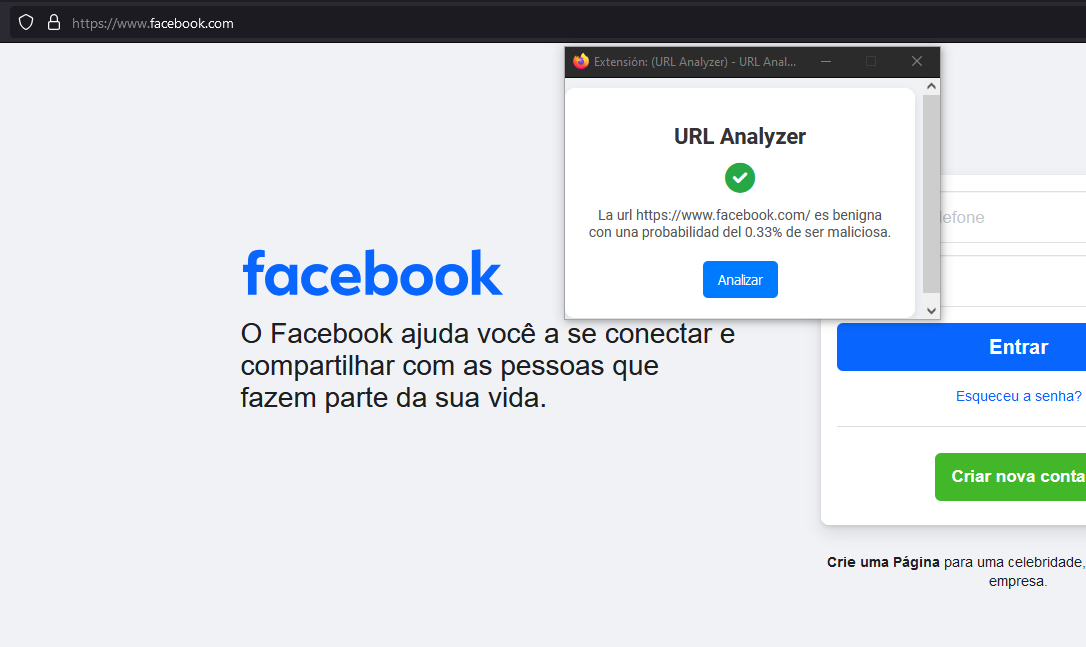
\includegraphics[width=0.7\textwidth]{image1.png}
    \caption{Análisis de la URL de Facebook.}
    \label{fig:facebook}
\end{figure}

\subsubsection*{Caso de Prueba 2: URL Maliciosa (Clon de Discord)}
\textbf{Descripción:}
Se utilizó una \gls{url} que imita la página de Discord, diseñada para engañar a los usuarios.

\textbf{Resultado:}
El análisis mostró que la \gls{url} \url{https://discord.zhangxinhe.com/} es maliciosa, con una probabilidad del 87.31\% de ser maliciosa.



\begin{figure}[H]
    \centering
    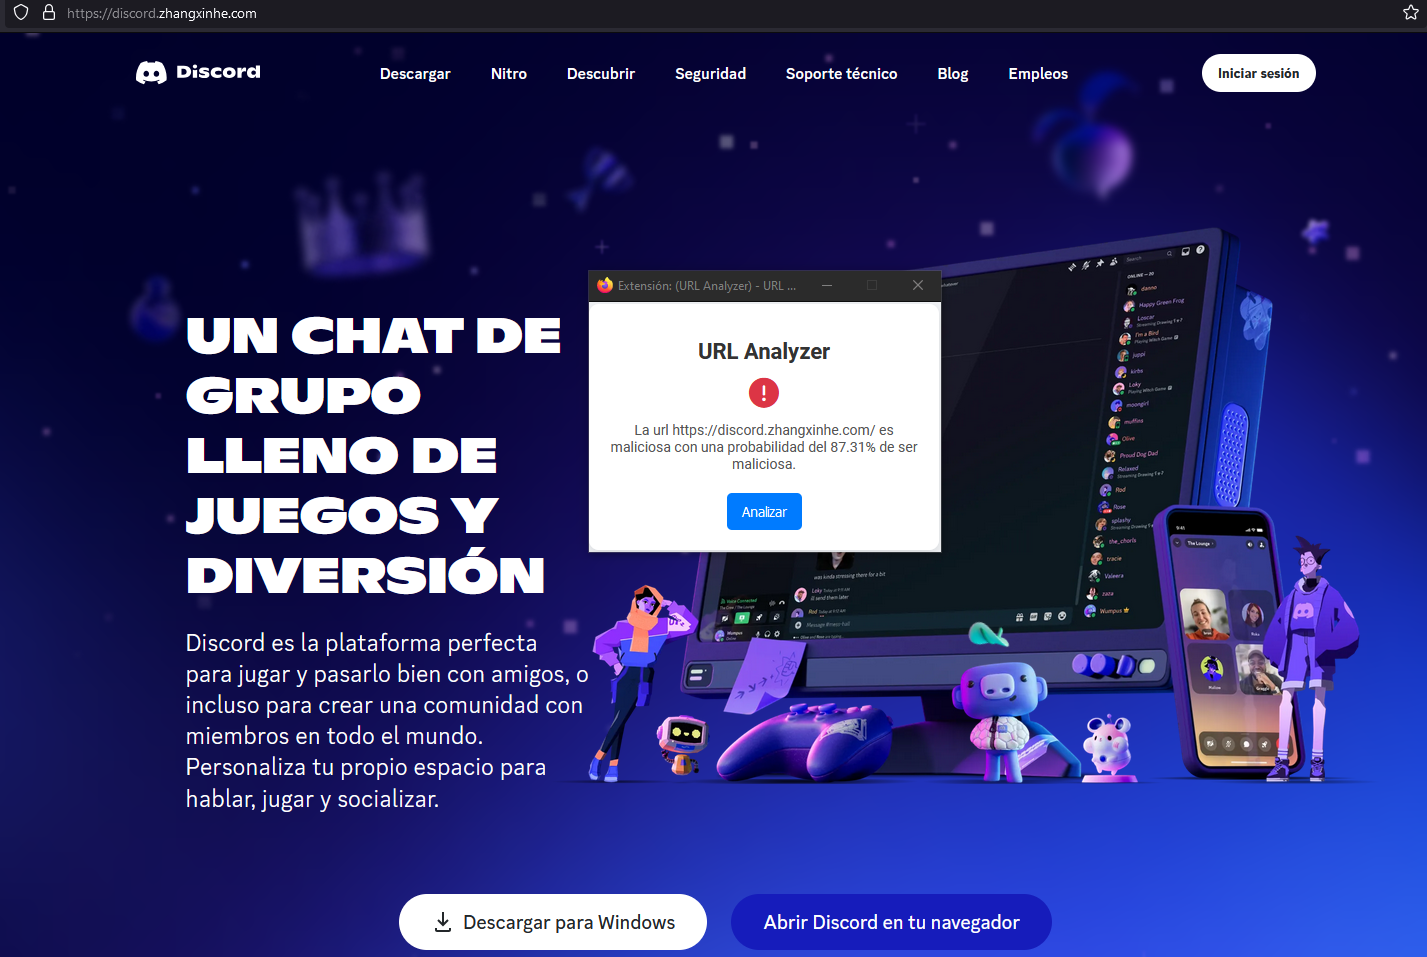
\includegraphics[width=0.7\textwidth]{image2.png}
    \caption{Análisis de una URL maliciosa clon de Discord.}
    \label{fig:discord_malicious}
\end{figure}

\subsubsection*{Caso de Prueba 3: URL Benigna (Discord)}
\textbf{Descripción:}
El plugin fue evaluado con la \gls{url} oficial de Discord, un servicio legítimo de chat y comunicación.

\textbf{Resultado:}
El análisis indicó que la \gls{url} \url{https://discord.com/} es benigna, con una probabilidad del 0.33\% de ser maliciosa.

\begin{figure}[H]
    \centering
    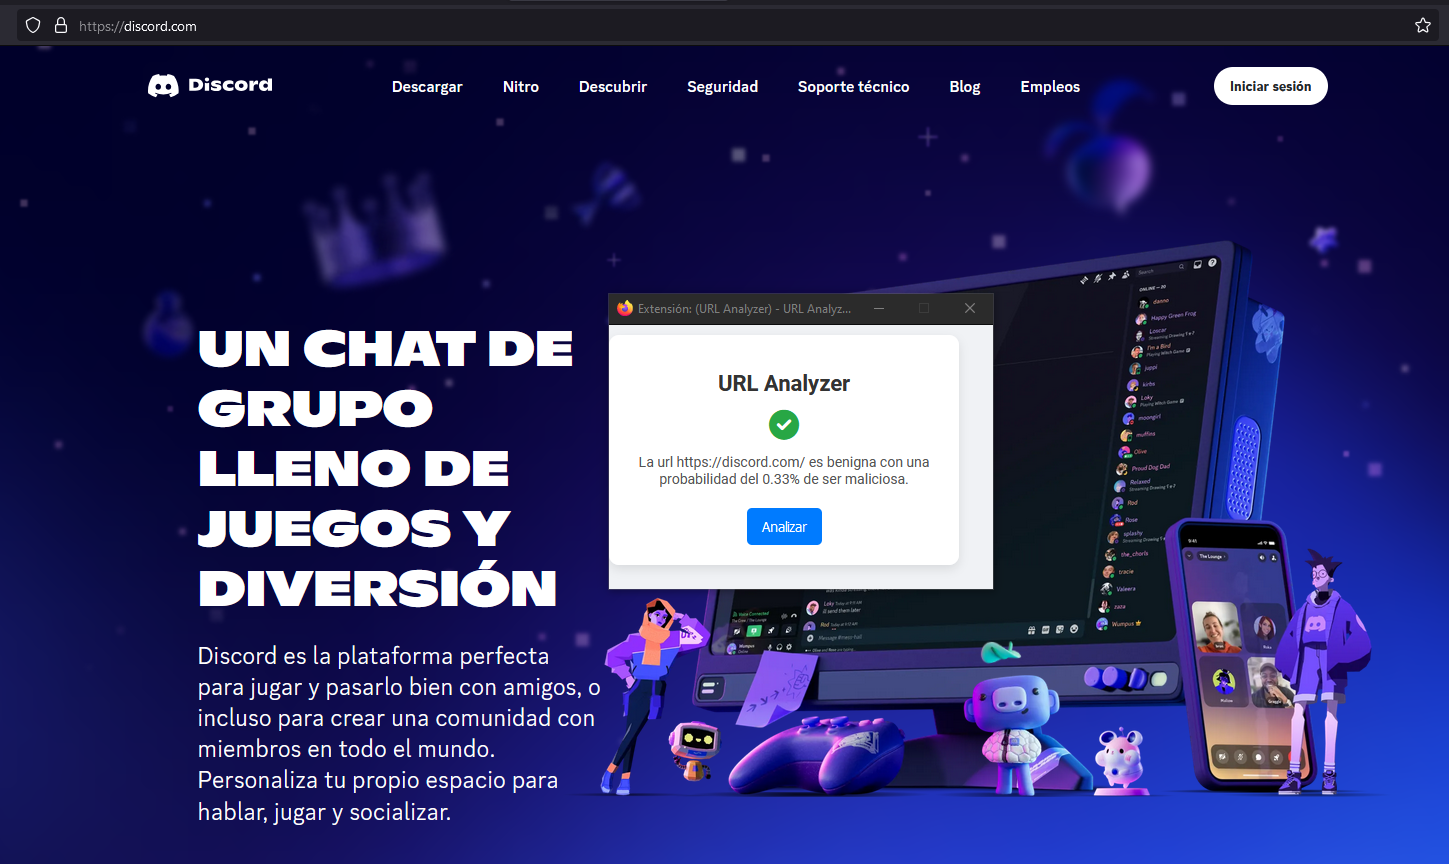
\includegraphics[width=0.7\textwidth]{image3.png}
    \caption{Análisis de la URL oficial de Discord.}
    \label{fig:discord}
\end{figure}

\subsubsection*{Caso de Prueba 4: URL Benigna (YouTube)}
\textbf{Descripción:}
Se probó el plugin con la \gls{url} de YouTube, una plataforma de videos conocida y segura.

\textbf{Resultado:}
El análisis mostró que la \gls{url} \url{https://www.youtube.com/} es benigna, con una probabilidad del 0.33\% de ser maliciosa.

\begin{figure}[H]
    \centering
    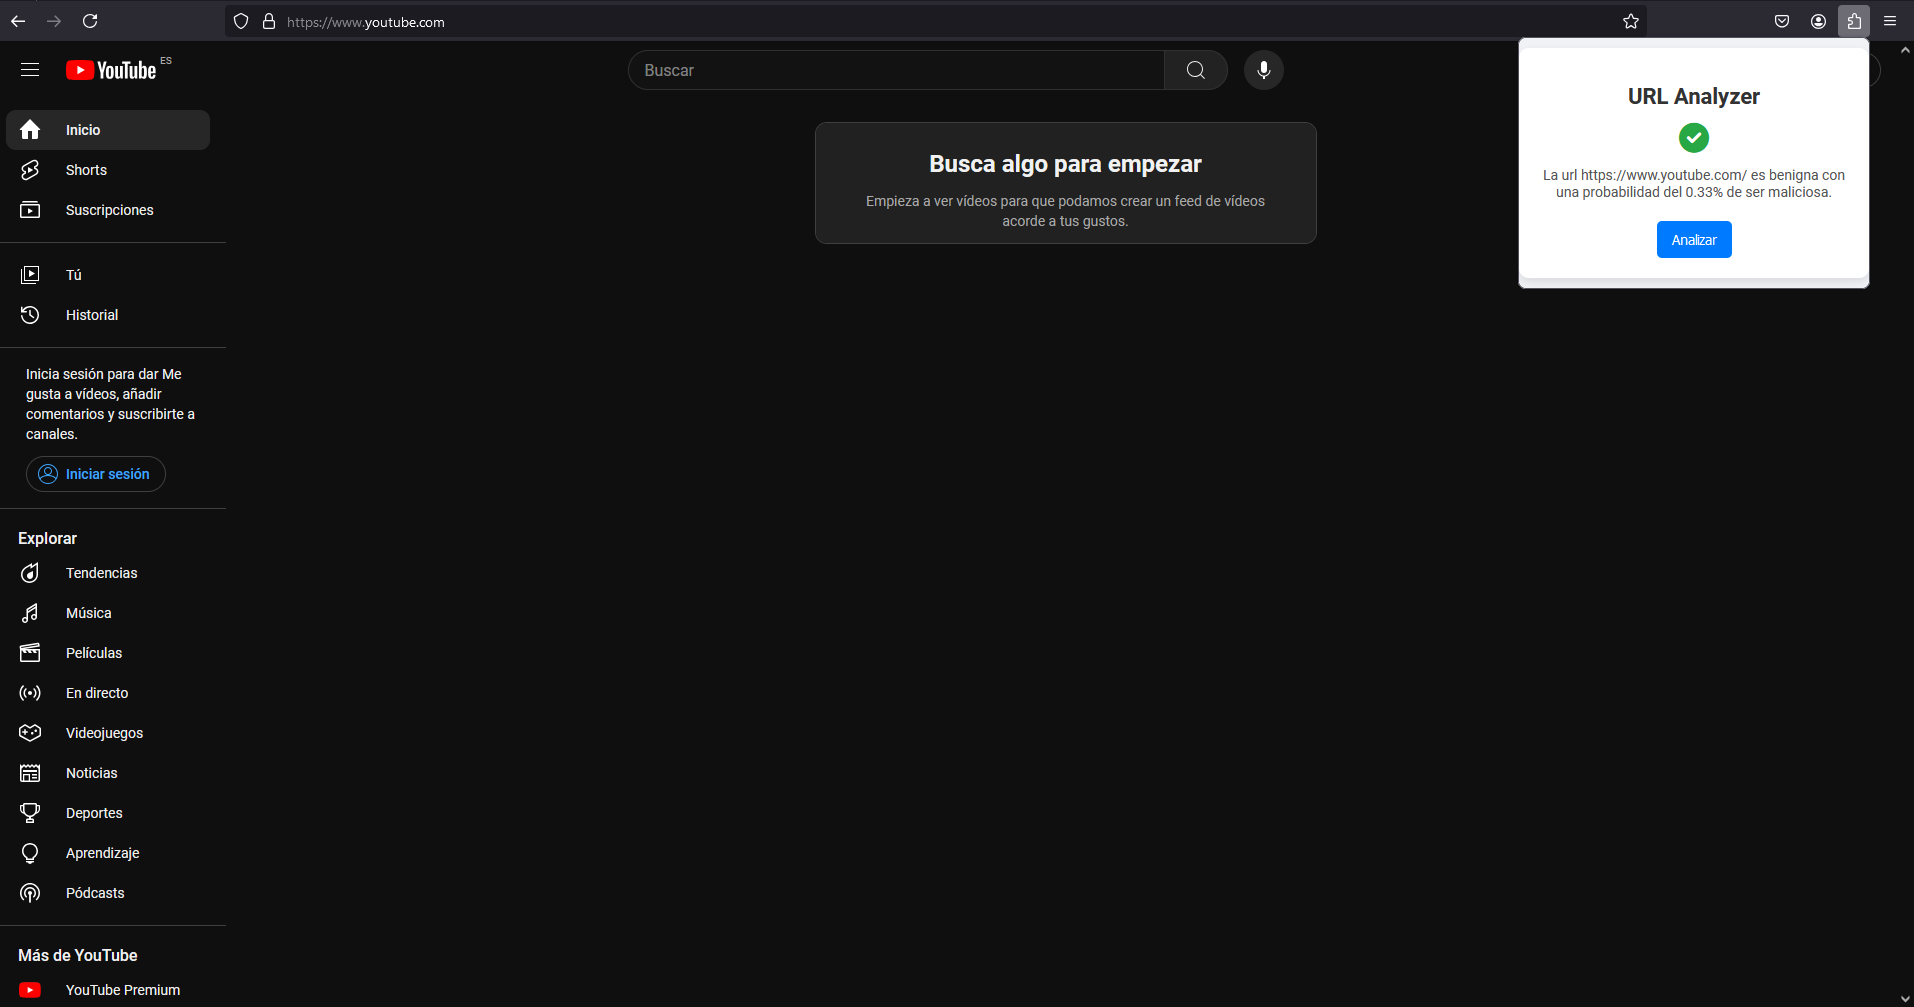
\includegraphics[width=0.7\textwidth]{image4.png}
    \caption{Análisis de la URL de YouTube.}
    \label{fig:youtube}
\end{figure}

\subsubsection*{Caso de Prueba 5: URL Maliciosa (Proxy de Discord)}
\textbf{Descripción:}
Se utilizó una \gls{url} que actúa como un proxy de Discord, diseñada para engañar a los usuarios.

\textbf{Resultado:}
El análisis indicó que la \gls{url} \url{https://discord-proxy.tassadar2002.workers.dev/} es maliciosa, con una probabilidad del 91.77\% de ser maliciosa.

\begin{figure}[H]
    \centering
    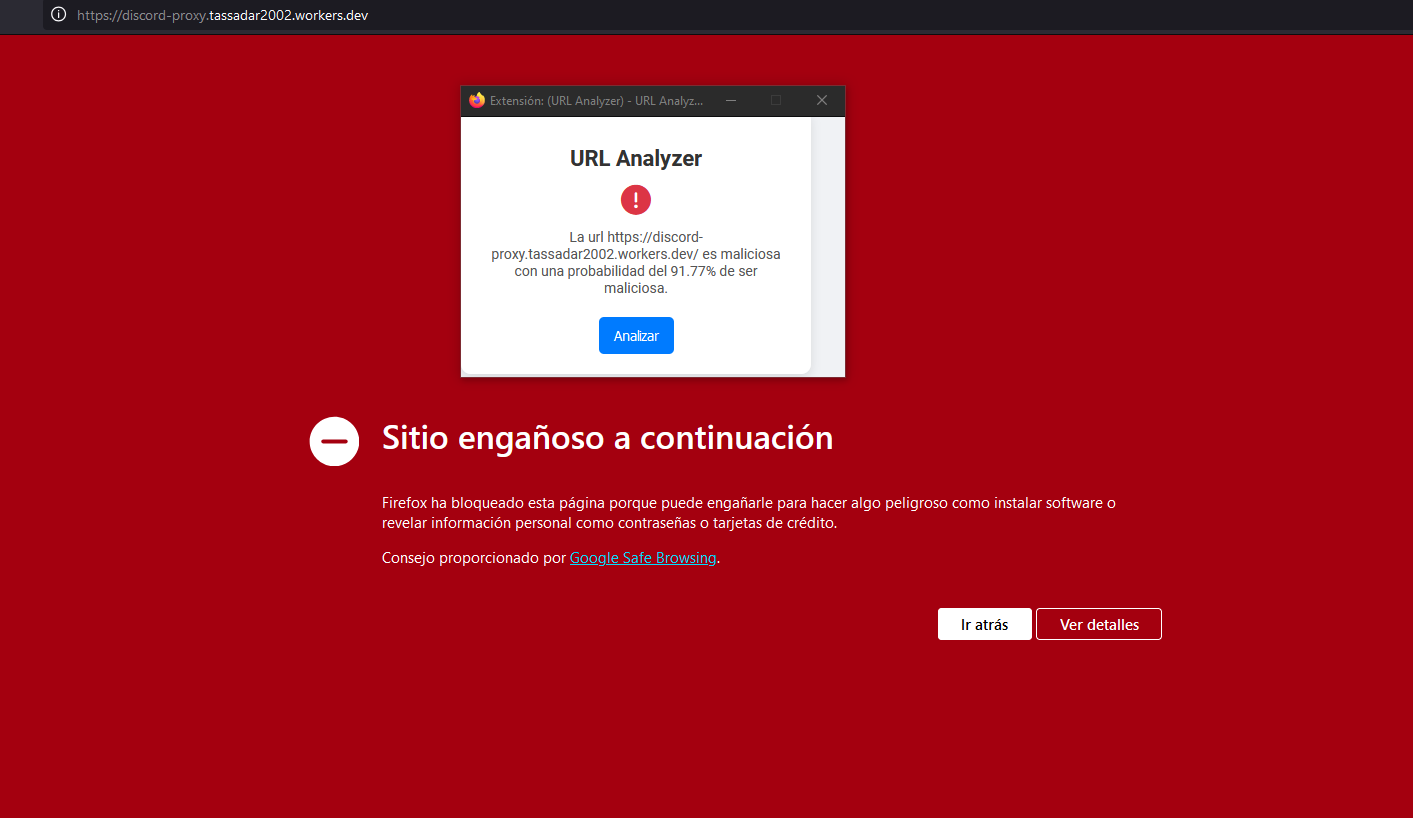
\includegraphics[width=0.7\textwidth]{image5.png}
    \caption{Análisis de una URL maliciosa proxy de Discord.}
    \label{fig:discord_proxy}
\end{figure}

\textbf{Nota:}
El navegador Firefox también detectó esta \gls{url} como maliciosa antes de que el plugin realizara su análisis, proporcionando una segunda capa de seguridad.


\subsubsection*{Caso de Prueba 6: URL Maliciosa Ignorando Advertencia del Navegador}
\textbf{Descripción:}
Se utilizó la misma URL maliciosa del Caso de Prueba 5, pero se ignoró la advertencia del navegador para entrar en la página.

\textbf{Resultado:}
El plugin siguió mostrando que la \gls{url} \url{https://discord-proxy.tassadar2002.workers.dev/} es maliciosa, con una probabilidad del 91.77\% de ser maliciosa.

\begin{figure}[H]
    \centering
    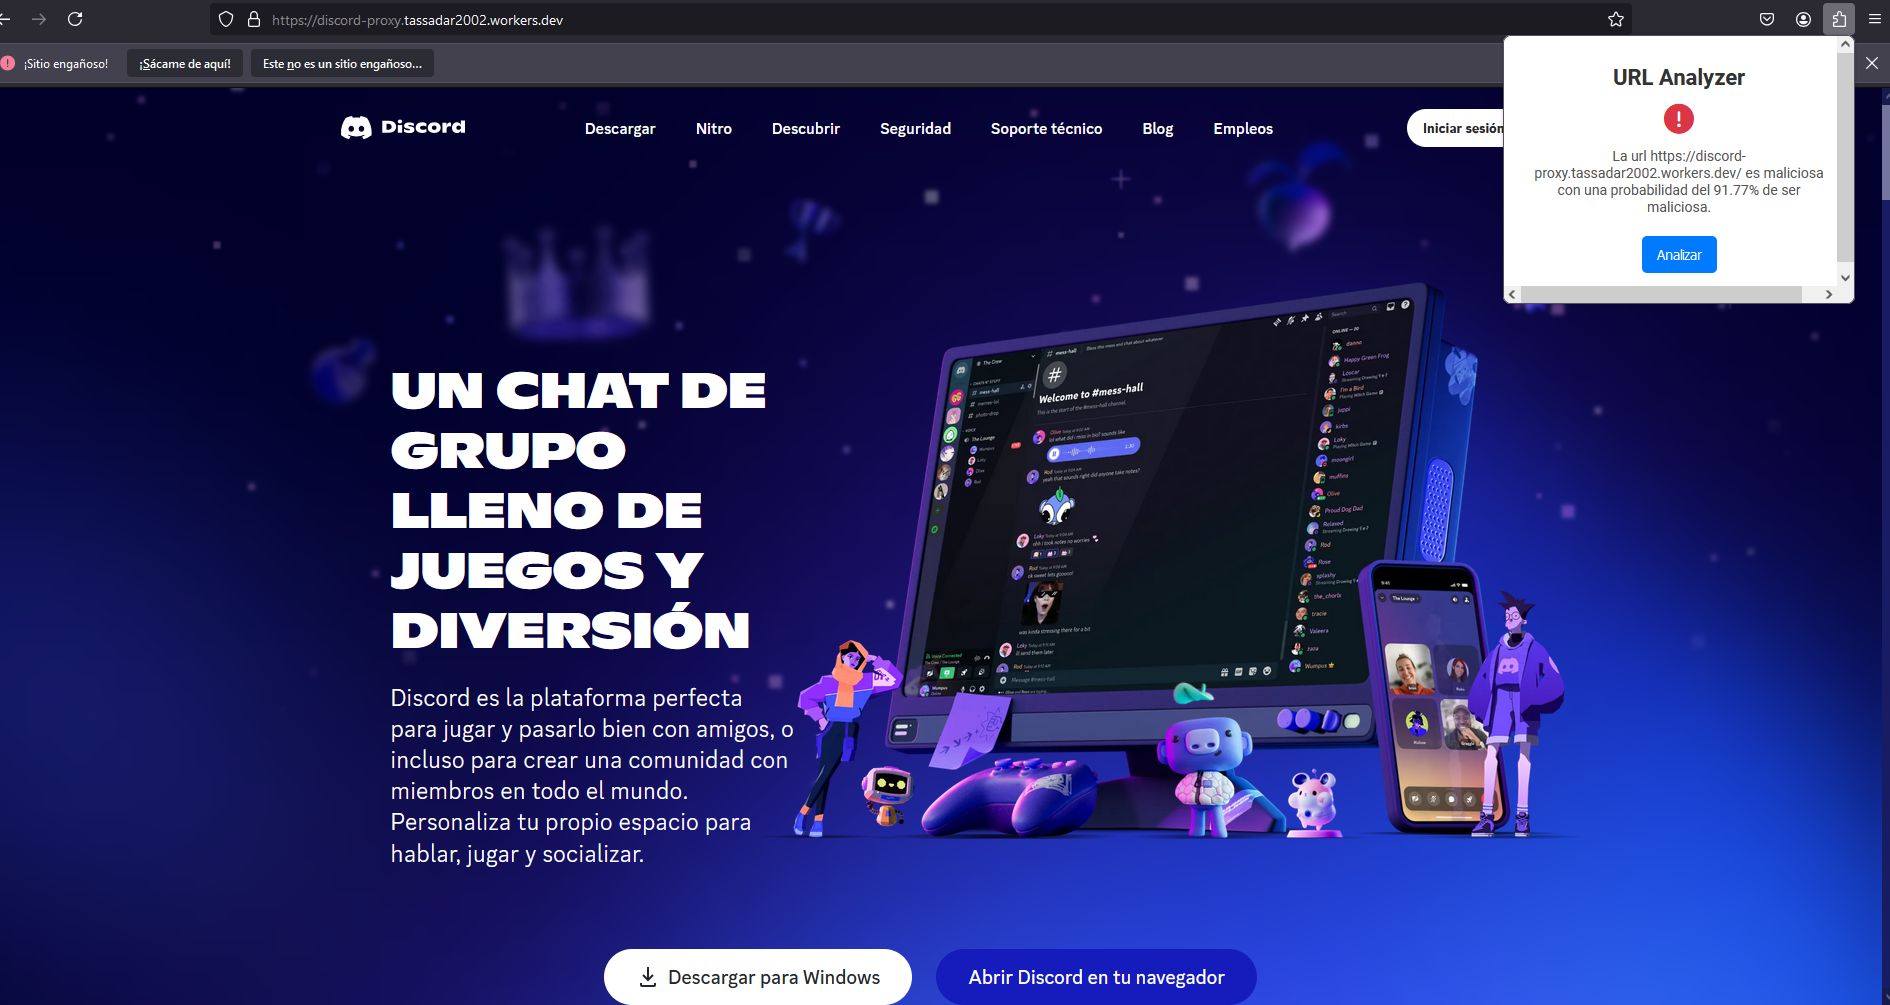
\includegraphics[width=0.7\textwidth]{image6.png}
    \caption{Análisis de una URL maliciosa ignorando la advertencia del navegador.}
    \label{fig:discord_proxy_ignored}
\end{figure}


\subsubsection*{Consideraciones Adicionales}
\begin{itemize}
    \item \textbf{Tiempo de Respuesta:} El tiempo promedio de análisis es de 5 segundos, lo que es razonable dado el nivel de análisis realizado.
    \item \textbf{Precisión:} El modelo de \textit{Machine Learning} utilizado por el plugin ha mostrado una alta precisión en la identificación de \glspl{url} maliciosas y benignas durante las pruebas.
    \item \textbf{Usabilidad:} La interfaz del plugin es intuitiva y fácil de usar, con notificaciones claras y accesibles para el usuario.
\end{itemize}

Para futuras mejoras, se podría considerar la optimización del tiempo de respuesta y la incorporación de funcionalidades adicionales basadas en feedback de los usuarios.
